\documentclass[onecolumn, draftclsnofoot, 10pt, compsoc]{IEEEtran}
\usepackage{graphicx}
\graphicspath{{./figures/}}

\usepackage{url}
\usepackage{setspace}
\usepackage{multicol}
\usepackage{pdflscape}
\usepackage{pdfpages}

\usepackage{geometry}
\geometry{textheight=9.5in, textwidth=7in}

% \overfullrule=2in

% 1. Fill in these details
\def \CapstoneTeamName{			Ground Station Software Team}
\def \CapstoneTeamNumber{		30}
\def \GroupMemberOne{			Kenneth Steinfeldt}
\def \GroupMemberTwo{			Christopher Pham}
\def \GroupMemberThree{			Corwin Perren}
\def \CapstoneProjectName{		OSU Robotics Club\\Mars Rover Ground Station}
\def \CapstoneSponsorCompany{	OSU Robotics Club}
\def \CapstoneSponsorPerson{	Nick McComb}



%Personal \newcommands

\newcommand{\functRequ}[4]{
\item #1%
\par
\begin{itemize}
\item \textit{Description:} #2.%
\item \textit{Rationale:} #3.%
\item \textit{Dependencies:} #4%
\end{itemize}
}



% 2. Uncomment the appropriate line below so that the document type works
\def \DocType{	%Problem Statement
				Requirements Document
				%Technology Review
				%Design Document
				%Progress Report
			 }
			
\newcommand{\NameSigPair}[1]{
  \par
  \makebox[2.75in][r]{#1} 
  \hfill
  \makebox[3.25in]{
      \makebox[2.25in]{\hrulefill} 
      \hfill
      \makebox[.75in]{\hrulefill}
  }
  \par\vspace{-12pt} 
  \textit{
      \tiny\noindent
      \makebox[2.75in]{} 
      \hfill
      \makebox[3.25in]{
          \makebox[2.25in][r]{Signature} 
          \hfill
          \makebox[.75in][r]{Date}
      }
  }
}
% 3. If the document is not to be signed, uncomment the command below
\renewcommand{\NameSigPair}[1]{#1}

%%%%%%%%%%%%%%%%%%%%%%%%%%%%%%%%%%%%%%%
\begin{document}
\begin{titlepage}
	\pagenumbering{gobble}
	\begin{singlespace}
		% 4. If you have a logo, use this includegraphics command to put it on the coversheet.
        \begin{minipage}{7in}
			\centering
			\hspace*{-.7in}
			$\vcenter{\hbox{
\includegraphics[height=4cm]{Oregon_State_College_of_Engineering_Logo}}}$
			\hspace*{.2in}
			$\vcenter{\hbox{
\includegraphics[height=2.5cm]{OSURCLogoOrange}}}$
		\end{minipage}

		\par\vspace{.35in}
		\centering
		\scshape{
			\huge CS Capstone \DocType \par
			{\large\today}\par
			\vspace{.5in}
			\textbf{\Huge\CapstoneProjectName}\par
			\vfill
			{\large Prepared for}\par
			\Huge \CapstoneSponsorCompany\par
			\vspace{5pt}
			{\Large\NameSigPair{\CapstoneSponsorPerson}\par}
			{\large Prepared by }\par
			Group\CapstoneTeamNumber\par
			% 5. comment out the line below this one if you do not wish to name your team
			\CapstoneTeamName\par 
			\vspace{5pt}
			{\Large
				\NameSigPair{\GroupMemberOne}\par
				\NameSigPair{\GroupMemberTwo}\par
				\NameSigPair{\GroupMemberThree}\par
			}
			\vspace{20pt}
            \begin{abstract}
			% 6. Fill in your abstract
            This document covers the design requirements for the OSU Robotics Club Mars Rover Team's Ground Station Software.
            It begins with details about why the software is necessary, and a general overview of what it needs to accomplish.
            We then go into further detail about what the specific functional requirements will be, how they relate to each other in terms of dependencies, and then end with stretch goals if there is extra time to complete them.

		\end{abstract}
		}
	\end{singlespace}
\end{titlepage}
\newpage
\pagenumbering{arabic}
\tableofcontents
\clearpage

% 8. now you write!
\section{Introduction}
\subsection{Purpose}
The purpose of this document is to formally define the characteristics of the software to be implemented. 
These requirements can then be used to determine if the software is complete once the project is done, while also serving as a reference during development.


\subsection{Scope}
We will be creating the "Mars Rover Ground Station" software package. 
This software will allow Rover team members to interact with the Oregon State University Robotics Club's Mars Rover for the purpose of a competition taking place in Utah during June of 2018. 
The software will provide Rover systems monitoring as well as control of drive and arm systems. 
During competition, the software will be run on a remote base station operated out of the Mars Desert Research Station or the back of a truck, allowing users to tele-operate the Rover during manned controlled missions, or to monitor progress during autonomous missions. 
Properly functioning and fully featured ground station software will be a major factor in the success of the Mars Rover during this competition.


\subsection{Definitions / Acronyms / Abbreviations}
\begin{itemize}
\item ROS - Robot Operating System
\item QT - A multi-platform GUI and application framework
\item GPS - Global Positioning Satellite 
\item User - Person operating rover from ground control station
\item GUI - Graphical User Interface
\item RTT - Round-trip Time, the length of time for a signal to be sent plus the length of the time it takes for an acknowledgement of the signal to be received.
\item Bogie - The individual wheels on the Rover, each with the ability to be driven independently.
\item IMU - Inertial Measurement Unit
\item FPS - Frames Per Second
\item CAD - Computer Aided Design
\end{itemize}


\subsection{Overview}
The remainder of this document consists of 4 sections and will describe the requirements that must be met in order for this project to be considered fully complete. The next section gives a description of the process. 
The fourth section describes the ground control software's functions, user characteristics, constraints, and assumptions and dependencies. 
The fifth section describes the specific requirements that must be met for the software to be a success.
Finally, stretch goals in the sixth section will describe hopeful, but not mandatory goals for the software.

\section{Description}
\subsection{Product Perspective}
This project interacts with and requires the Robotics Club's Mars Rover robotics vehicle in order to be useful.
If the Rover is not connected, the software will still be able to launch, but will not perform any useful functions until it has established a connection to the Rover.
In order to accomplish interaction with the rover, the ground station software will use ROS for primary functionality and feedback from the rover.


\section{Product Functions}
The ground control software will primarily accomplish two tasks:
\begin{itemize}
\item Provide Rover control to the user.
Direct rover control will be accomplished with two joysticks.
\item Enable and present rover feedback to the user.
The rover will send health and status information to the ground control station.
\end{itemize}


\subsection{User Characteristics}
Users of the Rover Ground Station software will comprise of Rover team leads and members.

\subsubsection{User Stories}
\begin{itemize}
\item User should be able to vary bandwidth as needed to adjust for latency at the event
\item User should be able view ground station UI on two HD monitors so that valuable competition time will not be spent switching between screens on a single monitor
\item User should be able to add way-points because way-points are needed to find useful points in the competition field and are necessary for autonomous navigation
\item User should be able to remove way-points because way-points may become unneeded or need to be reset for a new competition event
\item User should be able to edit way-points because there's a chance that the User may enter way-point details incorrectly and will need to change them
\item User should be able to change the order of way-points because we might need to traverse back to a location, or fix improperly entered way-points
\item User should be able to control the Rover by joysticks because that is the preferred way of controlling the Rover  
\item User should be able to select video streams because the Rover has more cameras than can be streamed at any one time, and being able to view any camera on demand will help the User drive the Rover and manipulate the arm
\item User should be able to view the pitch, yaw, roll of the Rover because we want to know if the rover is on an incline, decline, or about to tip over
\item User should be able to switch on and off autonomy because there are competition events that require autonomy and others that require manual control
\item User should be able to tell that autonomy is enabled because that alerts the User that they can no longer manually control the Rover
\item User should be able to tell that the rover has reached the final way-point after autonomy is enabled because that signals to the judges that the Rover has completed that competition event
\item User should be able to view how the arm joints are bent because that can show us if the arm is performing correctly
\item User should be able to control the arm because competition events require the use of a Rover arm
\item User should be able to view live logs from the Rover because that allows for debugging of hardware systems
\item User should be able to set the Rover speed limit so that the User can more easily drive the Rover over difficult terrain
\item User should be able to view the CPU usage because the User can use this information to tell if there is a software problem on the Rover or if the Rover is trying to process too much information
\item User should be able to view the memory usage because the User does not want the Rover to crash or slow down to unusable levels due to running out of memory
\item User should be able to view the drive usage because the User does not want the Rover to crash if the drive is full
\item User should be able to see the speed of the Rover because it can be used to determine if the Rover is driving at a speed that is reasonable for the current terrain
\item User should be able to see how accurate the GPS positioning is because at the competition there is a requirement to be a certain distance from an object
\item User should be able to see what heading the Rover is at because it allows for the User to know what direction to go
\item User should be able to see the maximum throughput of the network because it will allow for video stream quality to go up or down depending on the connection quality
\item User should be able to see the current latency because it will tell to the User or viewer how long a command will take to become action
\item User should be able to confirm connected devices because this will allow for debugging and checking of other connected devices
\end{itemize}


\subsection{Constraints}
Due to the nature of the Mars Rover project, there are multiple hardware and software constraints to ensure that the Ground Station software can properly communicate with the Rover. 
Additionally, the following constraints will help ensure future re-usability of the finalized software, which is a key goal of the Mars Rover team. 
\par
The software language allowed is the primary constraint for this project. 
Python 3 is required by the Mars Rover team as it maintains consistency with the software written on the Rover itself. 
The team also requires Python as it more easily allows future team members to reverse engineer code to be reused in future projects.
\par
Use of the QT application framework is another constraint placed by the Rover team in order to facilitate rapid prototyping of the user interface for this project. 
It will also allow for faster and easier modification both by future members of the team, and during competition as that has previously been necessary.
\par
The Rover internally uses ROS to handle routing and interpreting control and status information as well as video data. To be able to view this video data, status information, and to be able to send the Rover control information, this ground station software must also incorporate ROS.
\par
At a hardware level, the Rover team will be providing an Intel NUC desktop computer running Ubuntu 16.04 that the Ground Station software will need to be able to run on.
They will also provide two HD monitors, two USB joysticks, as well as a keyboard and mouse that will be used to view and interact with the software.


\section{Specific Requirements}
\subsection{User Interfaces}
Upon initial launch, the application should be in full-screen mode across both of the monitors. 
The left-hand screen will show navigation, Rover status, and miscellaneous Rover controls. 
The right hand monitor will show the three live video streams from the Rover. 
In the case that the software is started without a Rover to connect to, the software will display as-such and show placeholder information until such a connection is made.


\subsection{Functional Requirements}
\subsubsection{Statuses / Informational Readouts}
\begin{enumerate}
\functRequ{Rover Connection Status}
{This indicator will show a binary state of whether or not the Rover is currently connected}
{The Rover must be connected in order for most of the software aspects to function. 
It is also useful to tell when full network dropouts happen}
{None}

\functRequ{Joystick Connection Statuses}
{Status indicators will visually show binary states as to whether each of the two joysticks are currently connected}
{Both joysticks must be connected to drive the Rover}
{Rover Connection Status}

\functRequ{Rover Battery Status}
{This indicator will show the percentage of battery remaining on the Rover}
{The User should know how much battery is left to be able to determine remaining runtime and to diagnose other Rover errors}
{Rover Connection Status}

\functRequ{Rover Voltage Statuses}
{These indicators will show the major power rail voltages for the Rover}
{The User can use this information to diagnose faulty hardware and to determine cause if Rover systems become non-responsive}
{Rover Connection Status}
  
\functRequ{Bogie Connection Statuses}
{These indicators will show whether each of the six bogies are connected to the Rover}
{This will let drivers of the Rover know if a wheel has failed, which is a common occurrence}
{Rover Connection Status}

\functRequ{Arm Connection Status}
{This indicator will be a binary state of weather or not the mechanical arm is connected or not}
{This will show the User whether the arm is connected, and therefore whether they will be able to use the joysticks to control the arm}
{Rover Connection Status}

\functRequ{Arm Joint Positions}
{These indicators will show Rover Arm joint positions in terms of degrees or via visual relationships}
{These indications will help ensure the User knows where the Arm actually is, and whether it is being moved within its operating limits}
{Rover Connection Status, Arm Connection Status}

\functRequ{Camera Presence Statuses}
{This indicator will show which cameras on-board the Rover and connected and functional}
{The User can use such indicators to verify a failed camera for easy troubleshooting}
{Rover Connection Status}

\functRequ{IMU Status}
{This will indicate the pitch, yaw, and roll of the Rover}
{This can be used by the User to help navigate uneven terrain and to avoid flipping the Rover}
{Rover Connection Status}

\functRequ{Map Visualizer}
{This will display a map of  the current Rover location and surrounding areas}
{This can be used to see terrain maps of the area and to place useful way-point and autonomous navigation markers}
{Rover Connection Status}

\functRequ{Rover Computer Statuses}
{These indicators will show the current CPU, memory, and disk usage of the Rover's on-board computer}
{These can be used to ensure the Rover's processing computer is not overloaded.
It can also show potential software failures while serving as a useful indication that the connection to the Rover is stable}
{Rover Connection Status}

\functRequ{Current Radio Signal Strength}
{This indicator will display the strength of the connection between the Rover and ground station}
{The User can use this information to determine if the Rover is driving out of range to ensure a connection is not fully lost}
{Rover Connection Status}
  
\functRequ{Rover Network Potential Throughput}
{This indicator will show the maximum theoretical throughput in Kbps between the Rover and this software as provided by the Ubiquity routers}
{The User can use the information to help tune video bit-rates and resolutions to ensure the connection is not overloaded}
{Rover Connection Status, Current Radio Signal Strength, Rover RTT}

\functRequ{Rover RTT}
{This indicator will show how long in milliseconds the round trip time for a packet to and from the Rover takes}
{The User can use this information to help determine if delays in controls are due to network latency or other software error}
{Rover Connection Status, Current Radio Signal Strength}

\functRequ{Estimated Rover Distance}
{This indicator will show the distance from the Ground Station radio to the Rover radio, as calculated by the Ubiquiti radio systems}
{The User can use this information to help ensure they do not drive out of communications range}
{Rover Connection Status, Current Radio Signal Strength}

\functRequ{Rover Speed Limit}
{This display will show the Rover's speed limit in terms of 0 to 100 percent}
{During manual driving operations it is often useful to limit the max speed of the Rover.
A visual indication of this limit will help avoid confusion if the User forgets that a limit has been set, or if the limit is accidentally changed}
{Rover Connection Status, Rover Bogie Status}

\functRequ{Display Data Collection Sensors}
{Provide data displays for any scientific sensors attached to the Rover}
{During some competition phases, scientific sensors will be placed into the soil to gather scientific data.
This data needs to be sent back to the Ground Station so it can be recorded}
{Rover Connection Status}
\end{enumerate}

\subsubsection{Rover Control}
\begin{enumerate}
\functRequ{Rover Joystick Driving Control}
{When both joysticks are connected and the Rover is also connected, the joysticks can be used to drive the Rover}
{The joystick control is needed to be able to drive the Rover}
{Rover Connection Status, Joystick Connection Statuses, Bogie Connection Statuses}

\functRequ{Rover Joystick Arm Control}
{When both joysticks are connected, the Rover is connected, and the Arm is connected, the joysticks can be used to manipulate the Rover arm}
{During some competition events, the arm will need to be manipulated by the User to complete competition tasks}
{Rover Connection Status, Joystick Connection Statuses, Arm Connection Status}

\functRequ{Rover Speed Limit Control}
{When both joysticks are connected and the Rover is also connected, buttons or levers on a joystick may be used to adjust the max speed limit of the Rover}
{This quick adjustment is often needed to allow for finer control of the Rover over difficult terrain or when manipulating the Rover arm}
{Rover Connection Status, Joystick Connection Statuses, Bogie Connection Statuses}
\end{enumerate}

\subsubsection{Navigation}
\begin{enumerate}
\functRequ{GPS Status}
{This will show whether the GPS on the Rover is connected and whether it has GPS lock}
{This is needed to check to see if GPS is working and functioning properly}
{Rover Connection Status}

\functRequ{Rover Speed}
{This indicator shows how fast the Rover is moving in meters per second via the GPS}
{This will help the User ensure they are driving within the mechanical limits of the Rover}
{Rover Connection Status, GPS Status}

\functRequ{Rover Heading}
{This indicator will show what bearing the Rover is heading}
{The User can use this information to help navigate the competition course}
{Rover Connection Status, GPS Status}

\functRequ{GPS Satellites Connected}
{This indicator will show how many GPS satellites are currently active}
{This can help tell the User if the Rover is in a location that is bad for GPS reception, allowing them to drive to a better location before the GPS lock is lost}
{Rover Connection Status, GPS Status}

\functRequ{GPS Accuracy}
{This indicator will how accurate the current GPS location is in meters}
{This will allow the User to judge how much the GPS location of the Rover can be trusted, as well as giving useful information about how well the Rover might perform during the autonomous challenge}
{Rover Connection Status, GPS Status, GPS Satellites Connected}

\functRequ{Way-point Placement}
{Give the ability to place way-points on a map by GPS location, by current Rover location, or via manual GPS co-ordinate entry and add this way-point to a queue.
These way-points will also need to show up visually on the map}
{This will used to map out the course during the autonomous challenge as well as to place points of interest during manual driving events}
{Rover Connection Status, GPS Status, GPS Satellites Connected, Map Visualizer}

\functRequ{Way-point Editing}
{Allow for editing any way-point in the queue by drag and drop of the way-point, or via manual editing of the GPS co-ordinates}
{This will allow for easy adjustment of way-points if they were placed incorrectly}
{Rover Connection Status, GPS Status, GPS Satellites Connected, Way-point Placement, Map Visualizer}

\functRequ{Way-point Re-Ordering}
{Allow for changing the order of way-points}
{This will allow the User to skip unneeded way-points or fix incorrectly ordered way-points}
{Rover Connection Status, GPS Status, GPS Satellites Connected, Way-point Placement, Map Visualizer}

\functRequ{Way-Point Navigation Path}
{This should display the expected Rover navigational path when autonomous mode is active}
{This is useful to follow the progress of the Rover during the autonomy portion of the competition}
{Rover Connection Status, GPS Status, GPS Satellites Connected, Way-point Placement, Map Visualizer}

\functRequ{Active Way-point Selection}
{Allow for the selection of a way-point from the queue as currently active.
Setting the way-point active will update a "Heading To" indicator to help a User drive to the desired way-point}
{This is useful to make navigating to competition provided co-ordinates easier}
{Rover Connection Status, GPS Status, GPS Satellites Connected, Way-point Placement, Map Visualizer}

\end{enumerate}
\subsubsection{Autonomy}
\begin{enumerate}
\functRequ{Autonomy Switch}
{A toggle to enable and disable the Rover's autonomous mode operation}
{This is necessary to place the Rover into autonomous mode for that portion of the University Rover Challenge competition}
{Rover Connection Status}

\functRequ{Autonomy Indicator}
{An alert or indicator for when the Rover has reached its final way-point or has decided to stop}
{A University Rover Challenge requirement deems that this indicator is necessary to show to the judges when the Rover has completed its autonomy phase}
{Rover Connection Status, Autonomy Switch, Way-point Placement}
\end{enumerate}


\subsubsection{Video / Cameras}
\begin{enumerate}
\functRequ{Video Stream Displays}
{The software should show three video displays in terms of a primary, secondary, and tertiary display.
These displays will show streamed video feeds from cameras on the Rover and should be able to be individually disabled}
{The User will need video feeds from the Rover to navigate the competition course and to actuate the Rover arm}
{Rover Connection Status, Camera Presence Status}


\functRequ{Camera Source Selection}
{For the primary, secondary, and tertiary video displays provide controls to switch which Rover camera is currently active}
{During competition, the User will frequently be changing the active cameras to best navigate the competition course and interact with objects}
{Rover Connection Status, Camera Presence Status}

\functRequ{Camera Quality Adjustments}
{For the primary, secondary, and tertiary video displays provide controls to adjust the camera resolution and/or bit-rate}
{As the Rover gets farther away from the ground station, connection quality will diminish and require that the video stream qualities be lowered to ensure smooth Rover operation}
{Video Stream Displays}

\functRequ{Video Stream FPS Counters}
{These indicators will show the quality of the video streams by use of FPS counters for all three video streams}
{The User would want to know what the video stream FPS values are to determine if camera quality needs to be adjusted}
{Video Stream Displays, Rover Connection Status, Rover RTT}
\end{enumerate}


\subsubsection{Miscellaneous}
\begin{enumerate}
\functRequ{Log File Viewing}
{From within the software, the User must be able to view verbose logs of useful data}
{The User might want to access this stream to see any data that might help them troubleshoot problems such as faulty controls}
{Rover Connection Status}

\functRequ{UI Dark Theme}
{The software must be visually "dark" themed}
{The dark theme will help ease User eye strain and was also a client request}
{None}

\functRequ{Getting Started Document}
{A 1-2 page document describing general useful details for future Rover teams on where to begin for reusing the software}
{This was requested by the client}
{All Prior Requirements}

\functRequ{Quick Deploy Case}
{This requirement is to package all items necessary for the Ground Station to function in a quickly deployable case that can be set up in less than two minutes during competition setup time}
{Fast setup times will allow the User to spend extra time testing Rover communications during the setup phases of competition}
{All Prior Requirements}
\end{enumerate}


\section{Gantt Chart}
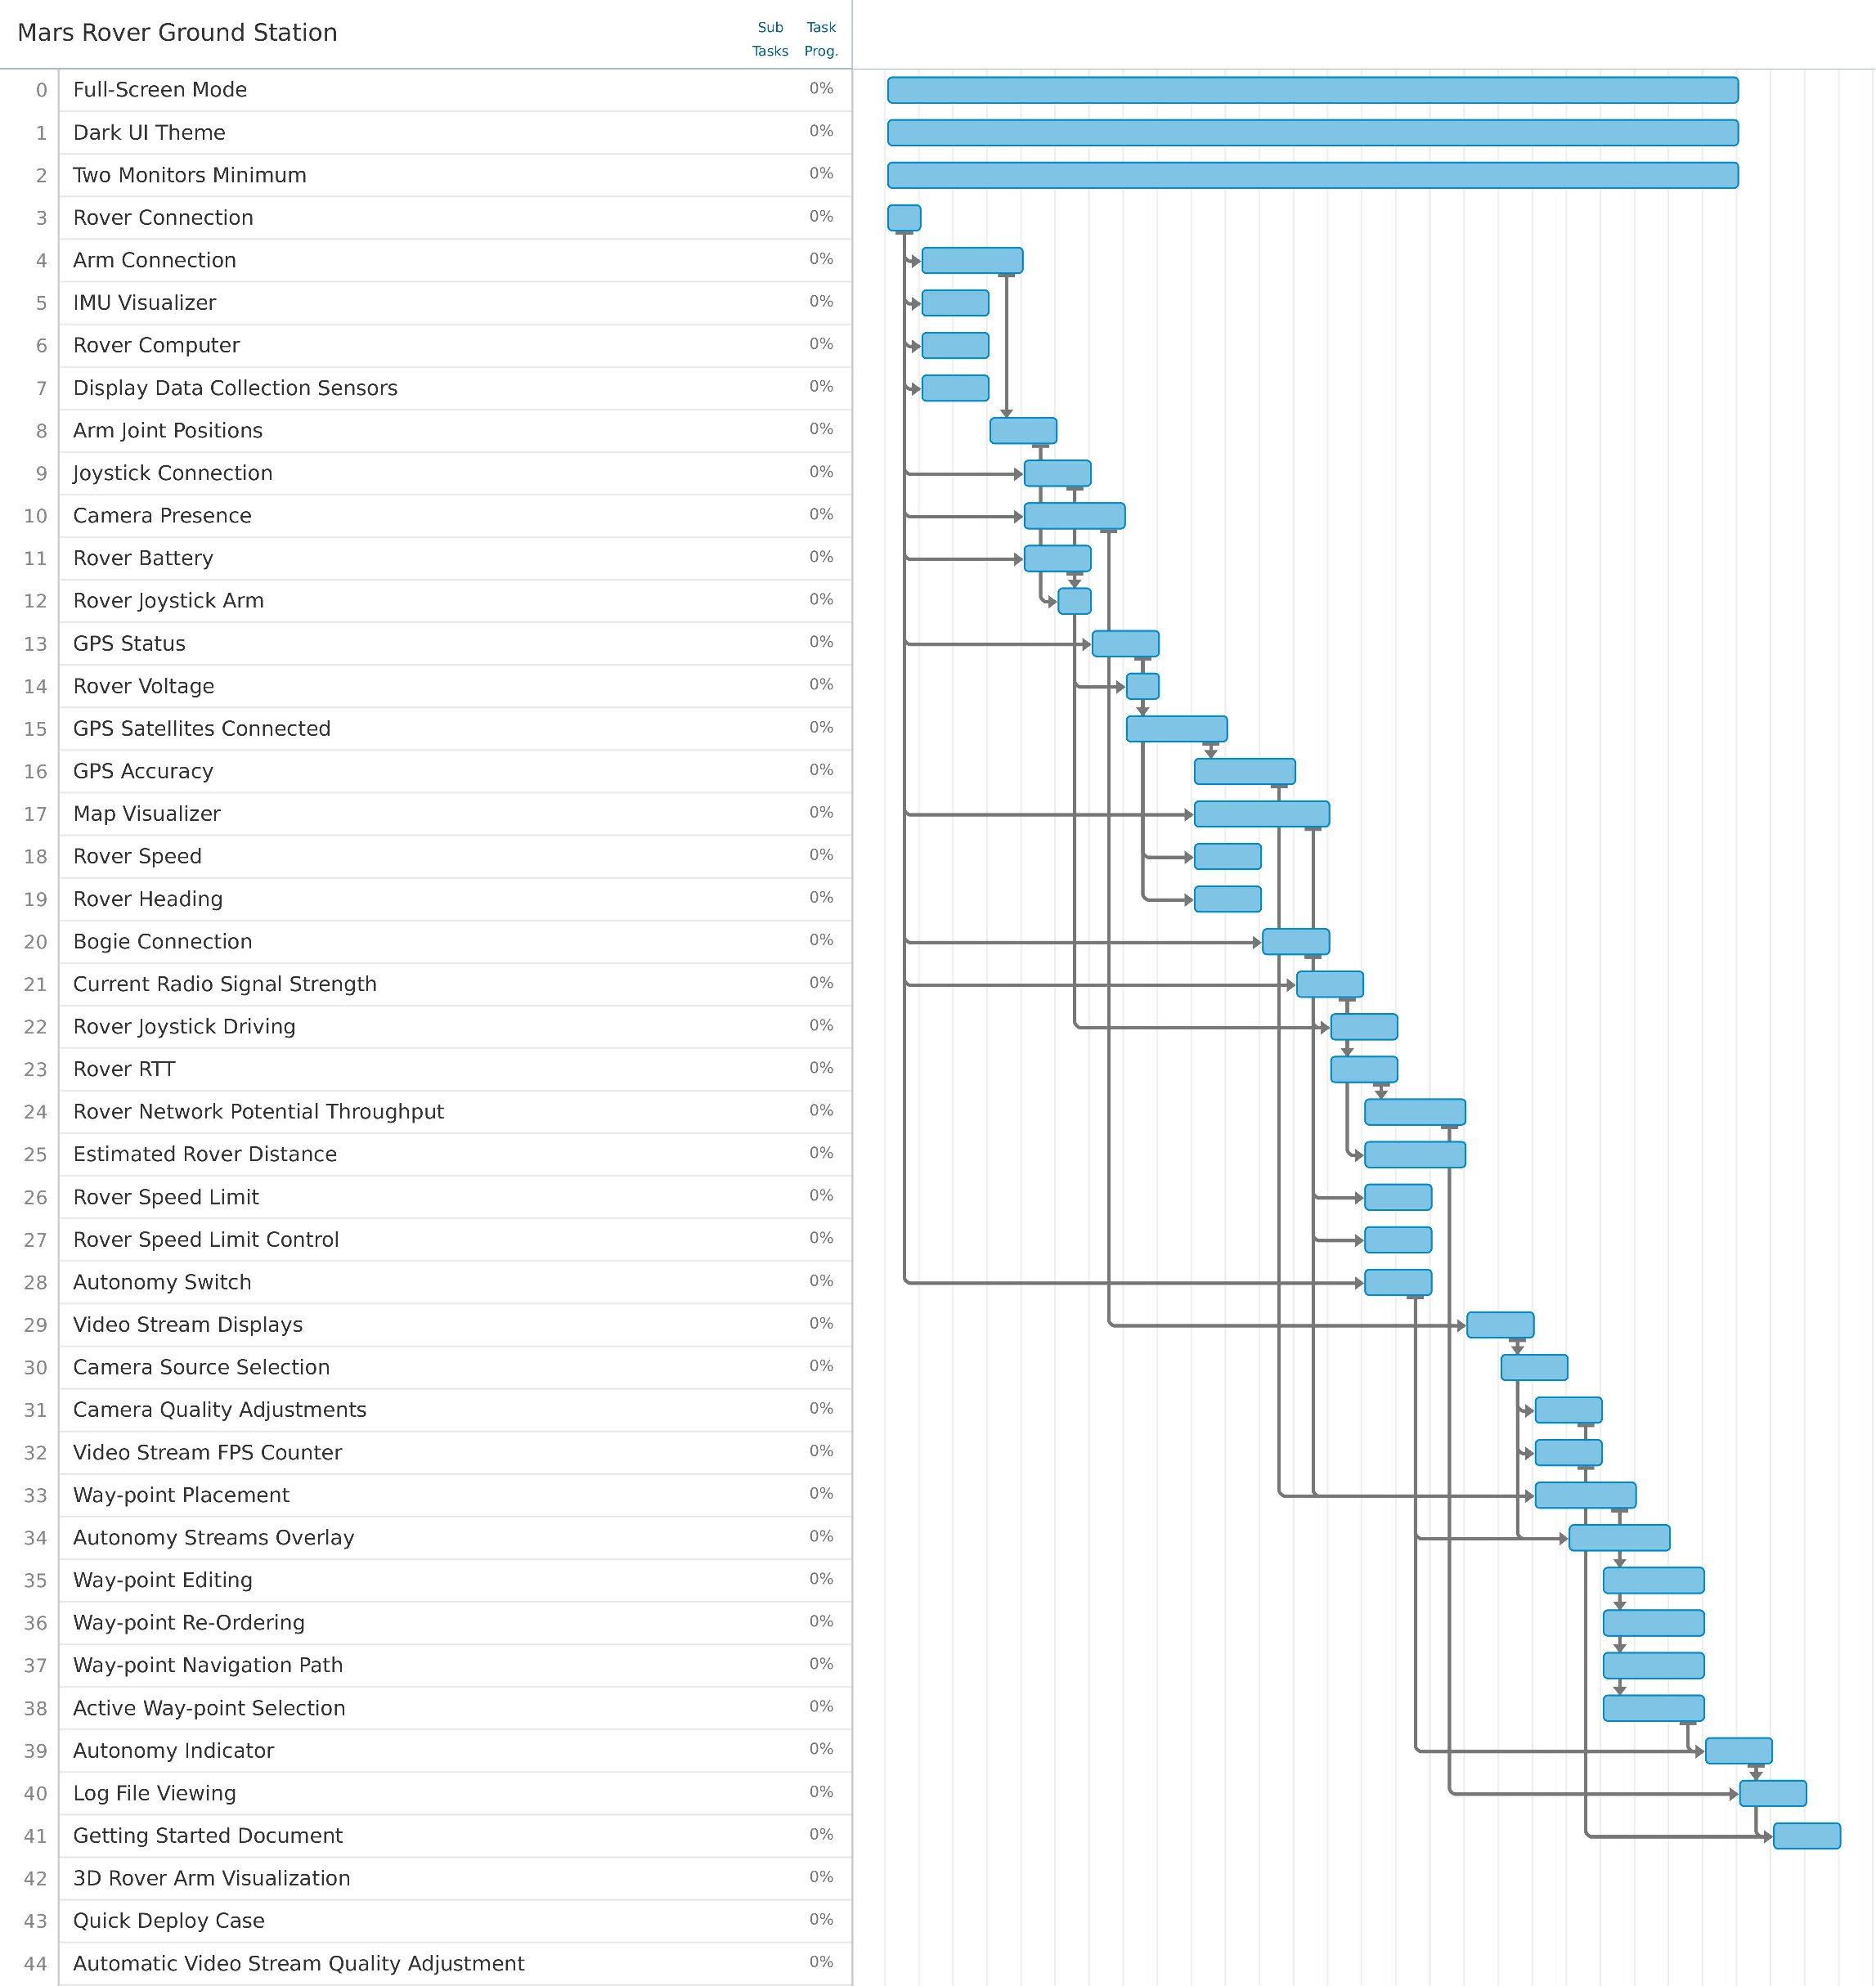
\includepdf{gantt_image}

\section{Stretch Goals}
\begin{enumerate}
\functRequ{Autonomy Streams / Overlay}
{This would display a specialty video stream either independently or via an overlay showing the course obstacles and/or features the Rover is detecting during autonomous mode navigation.
This would depend on the computational overhead remaining on the Rover processing computer}
{This would help the team judge autonomous navigational performance of the Rover}
{Rover Connection Status, Autonomy Switch}

\functRequ{3D Rover Arm Visualization}
{Represent the arm joint positions using a 3D CAD model of the arm}
{A 3D representation of the arm and its positioning will make it easier for the user to precisely use the arm to manipulate objects}
{Rover Connection Status, Arm Connection Status}

\functRequ{Automatic Video Steam Quality Adjustment}
{The software would automatically detect poor video quality through use of low FPS counts and/or high network latency and use this information to adjust video resolution and bit-rates to increase video stream FPS to reasonable levels}
{Automatic control of video stream quality would help the User avoid spending time adjusting values during valuable competition time}
{Video Stream Displays, Camera Quality Adjustments, Video Streams FPS Counters}

\end{enumerate}
\end{document}